\section{Introduction}
\label{sec:introduction}

\IEEEPARstart{R}{obotic} tool use on deformable and flowable media---scooping granular piles, pushing viscous pastes, transferring cohesive snow-like aggregates---requires adapting manipulation to hidden physical properties that are not visible in a single snapshot. Two materials that look nearly identical to a camera can differ by an order of magnitude in stiffness, cohesion, or flow resistance, and the manipulation strategy that succeeds on one of them can fail catastrophically on the other~\cite{huang2022plasticinelab,lin2022diffskill,shi2023robocook}. A robot that relies only on instantaneous observations therefore faces a dynamics-ambiguity problem: the same observed state can correspond to many distinct transition models.

A common response is to train reactive policies with domain randomization~\cite{tobin2017domain,peng2018sim2real} or to use a history-conditioned recurrent policy~\cite{hausman2018learning,xie2018learning}. These approaches trade breadth for depth---they spread the policy thin across many material instances without ever explicitly inferring what material the robot is currently manipulating. An alternative is discrete material classification followed by per-class policy routing~\cite{calandra2018more}, which requires a closed set of material labels and brittle perception. Neither strategy offers an explicit mechanism for the robot to \emph{ask the physics a question} before committing to a manipulation plan.

We take a different position: the information-gathering interaction is itself a physical intervention on the task state. Humans probe unfamiliar substances before picking them up and use the response to pick a grasp and a motion profile, but the probe can also compact, displace, or otherwise alter the material. We operationalize this intuition in \PTA{} (\cref{fig:hero}). \PTA{} is deliberately minimal: the probe is a fixed open-loop trajectory, the paired encoder is a small MLP, and the residual policy is standard PPO. The active component is the budgeted allocation of an initial interaction segment and the learned downstream use of its response; the probing action itself is not optimized as an information-gathering policy. The contribution of this paper is therefore empirical and diagnostic---a study of the sign pattern created when information gain and probe-induced state perturbation compete---not a new inference architecture.

\begin{figure*}[t]
    \centering
    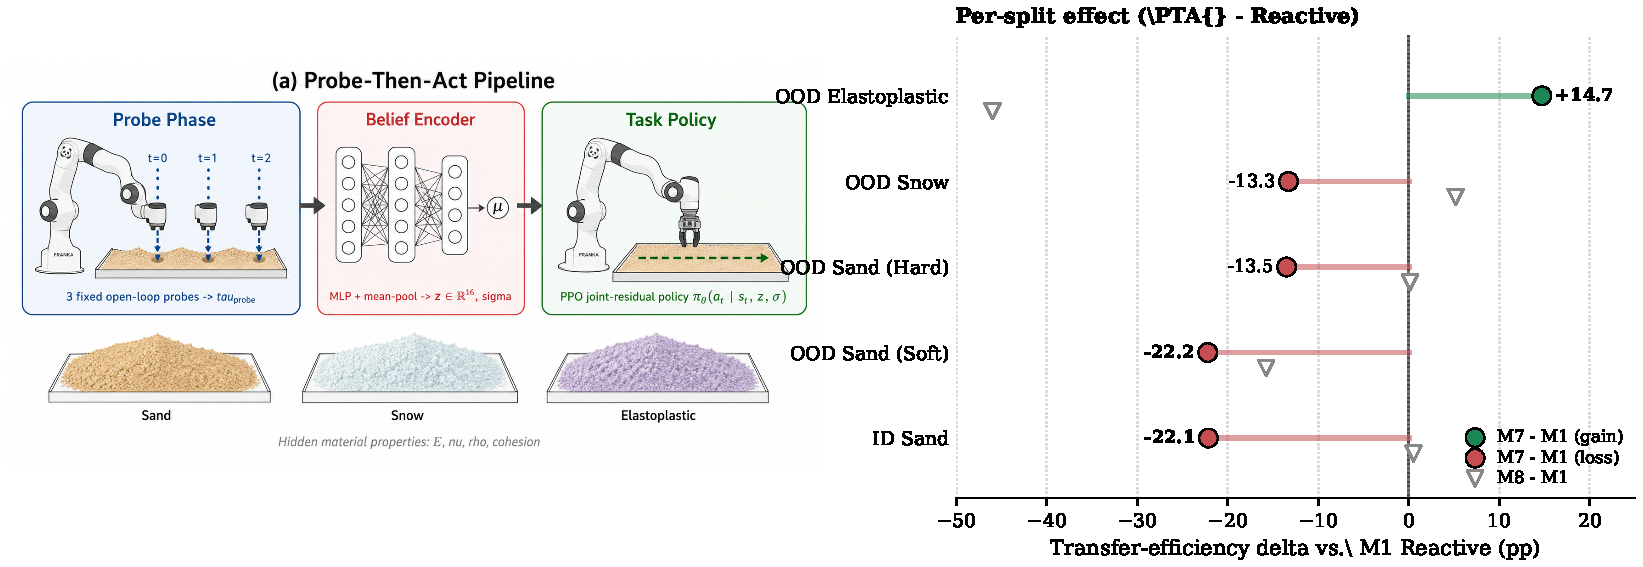
\includegraphics[width=0.98\textwidth]{figures/fig1_hero.pdf}
    \caption{\textbf{\PTA{} framework and per-split effect.} Left: schematic illustration of the two-stage architecture --- (i) the robot executes a short fixed open-loop probing phase, (ii) a paired encoder maps the probe trace to a latent task-conditioning vector $z$ with a scale output $\sigma$ (not a calibrated posterior), (iii) the task policy is conditioned on $(s_t, z, \sigma)$ to produce adaptive joint-space residual actions. Material piles below the schematic illustrate the three Genesis MPM families used in the benchmark; the schematic is for explanation and is not a Genesis render (Genesis renders appear in \cref{fig:scene_schematic}). Right: per-split transfer-efficiency delta of \PTA{} (M7) versus the matched reactive baseline (M1), in percentage points; hollow downward markers show the single-seed M8 privileged-parameter diagnostic delta. \PTA{} is positive on OOD elastoplastic ($+14.7$\,pp) and negative on ID sand, snow, Sand-Hard, and Sand-Soft ($-13$ to $-22$\,pp), while the M8 diagnostic is $-46$\,pp on elastoplastic. M1/M7 are means over 3 training seeds with 10 evaluation episodes per seed; this overview shows mean deltas only and the comparison is descriptive. Matched-seed dispersion is shown in \cref{fig:seeds}; absolute values for all three methods are in \cref{fig:main}.}
    \label{fig:hero}
\end{figure*}

\begin{enumerate}
    \item \textbf{Probe phase.} The robot executes a short, fixed open-loop sequence of exploratory contacts with the material while the task residual is held at zero. The resulting proprioceptive and aggregate-particle trace implicitly encodes the material's response to applied forces.
    \item \textbf{Encoder.} An MLP with mean-pooling maps the probe trace to a latent task-conditioning vector $z \in \R^{16}$ and a scale output $\sigma$. We refer to $(z, \sigma)$ as a ``belief'' for brevity, but the pair is not a calibrated posterior: there is no KL regularizer, prior, or auxiliary classification loss; in the matched protocol, the same paired encoder sidecar is saved and reloaded with the policy checkpoint.
    \item \textbf{Task policy.} A joint-residual PPO policy is conditioned on $(s_t, z, \sigma)$ and emits joint-space residuals on top of a scripted edge-push base trajectory. The base trajectory sidesteps differentiable-IK coupling artifacts we observed in the simulator~\cite{genesis2024}.
\end{enumerate}

\paragraph{The recoverable-deformation hypothesis.}
Probing is not free: every probe step displaces particles, breaks contacts, and consumes task time. We offer a physics-grounded interpretation of when this cost is likely to pay off, treated throughout as an \emph{interpretive hypothesis} rather than a demonstrated principle:
\begin{quote}
\emph{Active probing should be expected to help downstream manipulation only when the material's response to a probe is \textbf{recoverable}---the probed configuration relaxes back, on the task timescale, to a state the policy can still exploit---and to be net-negative when probe-induced perturbations are \textbf{irreversible}.}
\end{quote}
Elastoplastic media in our benchmark exhibit recoverable elastic rebound; granular sand (especially under low cohesion) exhibits irreversible rearrangement. Snow is cohesive in appearance but remains a negative case under contact loading, consistent with a persistent compacted or displaced region rather than a relaxed rebound. The hypothesis therefore anticipates, and our experiments are consistent with, gains on elastoplastic and losses on the persistent-perturbation splits.

\paragraph{Empirical evaluation.}
We evaluate \PTA{} on a reproducible cross-material edge-push benchmark in Genesis~\cite{genesis2024} spanning sand (granular, 32\% scripted transfer), snow (cohesive, 87\%), and elastoplastic medium with recoverable elastic rebound (70\%), plus two parameter-shifted sand variants. The 55-percentage-point scripted-transfer spread is discriminative by design. All methods are trained on the hardest split (sand) only and evaluated zero-shot on the other four, so the policy and paired latent input are evaluated in extrapolation rather than interpolation over a labeled material mix.

On the elastoplastic split, \PTA{} achieves $60.7$\% transfer versus $46.0$\% for a matched reactive PPO baseline (M1)---14.7pp absolute, 32\% relative---accompanied by a 14.7pp reduction in spillage (39.3\% vs.\ 54.0\%; \cref{tab:main_results}, \cref{fig:main}). A separate corrected matched-encoder audit removes a legacy encoder-mismatch concern: seed 42 passes the matched audit with $96.8$\% transfer, and six matched M7 seeds average $93.5$\% transfer on elastoplastic versus $39.4$\% for six reactive seeds (4/6 matched-seed wins, two near ties; \cref{tab:matched_encoder_audit}). Matched ablations clarify the source of this improvement: removing the probe drops transfer by 27.6pp and falls below M1, while removing only the encoder output drops 14.4pp from full \PTA{} and returns to roughly M1-level transfer (\cref{tab:ablation}). On ID sand, snow, and two sand parameter shifts, \PTA{} underperforms by 13--22pp, including a 22pp loss on in-distribution sand. We treat this as an observed sign pattern: active probing is positive on the recoverable split and negative where the probe-induced perturbation persists. A complementary observation: a single-seed privileged-parameter diagnostic (M8) that receives ground-truth material parameters scores 0\% transfer on elastoplastic while remaining strong elsewhere. In our sand-only-trained, residual-control setup, a passive parameter vector did not unlock a learned response curve for elastoplastic rebound while a probe-induced response did.

\paragraph{Contributions.} We make three contributions, framed as empirical and diagnostic:
\begin{enumerate}
    \item A \textbf{diagnostic sign pattern}: on a discriminative cross-material benchmark, a minimal probe-then-act policy improves the recoverable elastoplastic split (+14.7pp transfer, $-$14.7pp spill, +16.7pp success) while underperforming by 13--22pp on ID sand, snow, and two sand parameter shifts; a corrected matched-encoder six-seed audit strengthens the elastoplastic direction (+54.2pp mean transfer, 4/6 wins), and matched ablations show that skipping the probe falls below the reactive baseline while dropping only the encoder returns to roughly baseline transfer.
    \item A \textbf{recoverable-deformation hypothesis}, offered as a physically motivated candidate boundary condition for active probing and a testable prediction for future work on additional viscoelastic and compacting granular media.
    \item A \textbf{reproducible cross-material benchmark} in Genesis with five splits (55pp of scripted-transfer spread), standardized 3-seed protocol, per-seed metrics, and ablation infrastructure; code and seeds will be released upon acceptance.
\end{enumerate}

\paragraph{Scope of claims.}
\PTA{} as evaluated here uses a fixed open-loop probe, observations that include simulator-derived aggregate-particle statistics, and a matched task-conditioning latent without calibration or material-label supervision; all training is on sand. This scopes the paper as a \emph{diagnostic} study of when a minimal probe-conditioned policy helps and as a benchmark for future sensing and robustness work.

The rest of the paper is organized as follows. \cref{sec:related} positions our work against active perception, deformable manipulation, system identification, and multi-physics benchmarks; \cref{sec:method} formalizes \PTA{}; \cref{sec:experiments} describes the benchmark and evaluation; \cref{sec:results} reports the main results and ablations; \cref{sec:discussion,sec:conclusion} discuss scope, limitations, and conclude.
